\documentclass[twocolumn,superscriptaddress,aps]{revtex4-1}

\usepackage[utf8]{inputenc}

\usepackage{amsfonts}
\usepackage{amssymb}
\usepackage{amsmath}
\usepackage{amsthm}

\usepackage{bbold}
\usepackage{bm}
\usepackage{graphicx}
\usepackage{color}
\usepackage{hyperref}
\usepackage{enumitem}

\hypersetup{
  colorlinks,
  citecolor=blue,
  linkcolor=red,
  urlcolor=blue}
\DeclareMathOperator*{\argmin}{arg\,min}
\def\changemargin#1#2{\list{}{\rightmargin#2\leftmargin#1}\item[]}
\let\endchangemargin=\endlist 


\begin{document}


% ==============================================================================

\title{\Large{INFO8004: A review of Machine Theory of Mind}}
\vspace{1cm}
\author{\small{\bf Aurélien Werenne}}
\affiliation{\texttt{awerenne@student.uliege.be} (\texttt{s110995})}

\maketitle

% ==============================================================================


\section*{Abstract}
\begin{changemargin}{0.55cm}{0.55cm} 
Artificial Intelligent agents are becoming increasingly important parts of our daily lives. From drones to smart home assistants, human-machine interaction has made enormous progress in the last decade. Nevertheless, we are still very far from smooth human-level interactions. How can agents be constructed in order to evolve safely in complex multi-agent environments? In particular, in environments where each agent (natural or artificial) potentially has different goals and beliefs about the world. The paper \textit{Machine Theory of Mind} \cite{Tomnet} is an attempt to make a step towards a solution to this problem. In this review paper we i) present the experiments and results of \cite{Tomnet} ii) discuss its strength and limitations iii) explore possible applications.
\end{changemargin} 

\section{Introduction}

\noindent For the course, Advanced Machine Learning (INFO8004), my assignment is to analyze and summarize the work done by Neil C. Rabinowitz et al. \cite{Tomnet}, where they propose a neural network able to model agents it encounters based solely on observations. This review paper is organized into three parts. First, in section \ref{sec:background} the necessary background is shortly explained. Then the experiments and results of \textit{Machine Theory of Mind} are described in section \ref{sec:machinetom}. And finally, we discuss the limitations of the paper.


\section{Background}\label{sec:background}

\noindent \textbf{Theory of Mind} \\[0.15cm]
In 1978, Premack \& Woodruff made a brilliant piece of work \cite{Woodruff} by demonstrating that chimpanzees are able to infer the behaviour of other individuals, a concept defined as the Theory of Mind (ToM). This ability is only observed in humans, apes and some species of birds. In general, individuals are said to have a Theory of Mind if they are able to represent the mental states of others, including their desires, beliefs and intentions. \\

\indent Byom \& Mutlu \cite{Mutlu} identified that a ToM consists out of three mechanisms. First, the observer needs to be able to extract knowledge of the shared context with the observed agent. The second mechanism is the perception of social cues, gazes and emotion recognition. Understanding sarcasm is one example of the utility of social cues interpretation. As Williams et al. reported \cite{williams}, speakers in Western cultures tend to look away from their partners while making sarcastic comments, signaling that the speaker does not actually believe what he or she is saying. Lastly, an agent with a ToM needs to be able to interpret other's actions: inferring a character's belief based on observations of their actions.\\

\noindent \textbf{Sally-Anne test} \\[0.15cm]
A common psychological test used to evaluate a person's social cognitive ability to attribute (false) beliefs to others is the Sally-Anne Test (SAT, \cite{wimmer}), which is in the form of a story-telling:
\begin{enumerate}
\item Introduction of two dolls, Sally and Anne
\item Sally takes a ball and hides it in the white box
\item She then leaves the room 
\item While she is away, Anne takes the ball out of the white box and puts it in the black box
\item Sally comes back into the room. The belief question is then asked to the tested person: Where will Sally look for her ball?
\end{enumerate}
The experiments of increasing complexity performed by Rabinowitz and colleagues built-up towards a simplified simulation of the Sally-Anne test. \\

\noindent \textbf{Meta-Learning} \\[0.15cm]
Meta-learning \cite{Schmidhuber} is an area of research that tackles the problem of \textit{learning to learn}. The goal is to design models that can learn new skills or rapidly adapt to new environments with minimal training examples. Formally, the learning problem at training time can be written as
\begin{equation}
\theta^* = \argmin_\theta \mathbb{E}_{\mathcal{D} \sim p(\mathcal{D})}[\mathcal{L}_\theta(\mathcal{D})]
\label{eq:meta}
\end{equation}
where $\mathcal{D}$ is a sampled dataset from the task distribution. In other words, the optimization process finds a \textit{prior} on the parameters that are good in general on new sampled datasets. During test time, the parameters are updated with respect to the sampled dataset, which can be seen as the \textit{posterior} step in the Bayes update.

\section{Machine Theory of Mind}\label{sec:machinetom}
The objective of the paper \cite{Tomnet} is to build an Artificial Theory of Mind, where the \textit{observer} infers the mental states of other agents. More specifically, the observer will get access to a set of behavioural traces of a novel agent, and asked to make predictions of the agent's future behaviour. \\

One of the main insights of this work is to consider this challenge as a meta-learning problem. Two components of the observer are introduced: a \textit{general} and an \textit{agent-specific} Theory of Mind. The general ToM are the learned weights of the network, encapsulating the common behaviour of all agents in the training set. On the other hand, the agent-specific ToM is formed from observations about a single agent at test time. \\

The environments considered during the experiments are all gridworlds with a common action space (up/down/left/right/stay), deterministic dynamics, and a set of consumable objects (see Fig.1).\\

\begin{figure}[!htb]
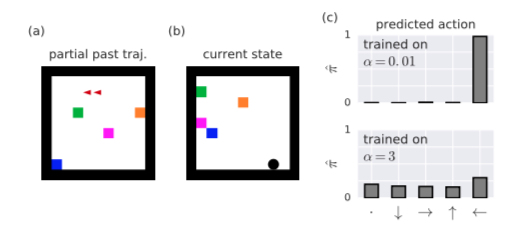
\includegraphics[width=\linewidth, height=\textheight, keepaspectratio]{figs/exp1-1}
\label{fig:exp11}
\caption{\textbf{Example gridworld in which a random agent acts.} Description copied from original paper. \textbf{(a)} Example past episode. Coloured squares indicate objects. Red
arrows indicate the positions and actions taken by the agent. \textbf{(b)} Example query: a state from a new MDP. Black dot indicates
agent position. \textbf{(c)} Predictions for the next action taken by the agent shown in (a) in query state (b). Top: prediction from ToMnet trained on agents with near-deterministic policies. Bottom: prediction from ToMnet trained on agents with more stochastic policies.}
\end{figure}

\noindent \textbf{Framework} \\[0.15cm]
The authors propose a simple yet powerful general framework to train and create a ToM intelligence. The task is formalized as a partially observable Markov decision process (POMDP) $\mathcal{M}_j = (S_j,A_j,T_j)$ with $S_j$, state spaces, $A_j$, action spaces and $T_j$ the transition probabilities. Notably, the authors make the uncommon clever choice to associate the reward to the agent instead of the environment.\\

The agents are defined as $\mathcal{A}_i$, with observation spaces $\Omega_i$, conditional observation functions $\omega_i(\cdot):S\rightarrow\Omega_i$, reward functions $R_i$, discount factors $\gamma_i$, and resulting policies $\pi_i$.\\

In turn, the observer who makes potentially partial and/or noisy observations of agents' trajectories, via a state-observation function $\omega_i^{(\text{obs})}(\cdot):S\rightarrow\Omega_i^{(\text{obs})}$ and an action-observation function $\alpha_i^{(\text{obs})}(\cdot):A\rightarrow A_i^{(\text{obs})}$. Thus, if agent $\mathcal{A}_i$ follows its policy $\pi_i$ on POMDP $\mathcal{M}_j$ and produces trajectory $\tau_{ij}^{(\text{obs})} = \{(s_t, a_t)\}_{t=0}^T$, the observer would see $\tau_{ij}^{(\text{obs})} = \{(x_t^{(\text{obs})},a_t^{(\text{obs})})\}_{t=0}^T$, where $x_t^{(\text{obs})} = \omega^{(\text{obs})}(s_t)$ and $a_t^{(\text{obs})} = \alpha^{(\text{obs})}(a_t)$.\\

\noindent \textbf{Model} \\[0.15cm]
The ToMnet (see Figure 2) is composed of three modules: a \textit{character net}, a \textit{mental net}, and a \textit{prediction net}. The goal of the character net is to characterise the presented agent, by parsing observed past episode trajectories, $\{\tau_{ij}^{(\text{obs})}\}_{j=1}^{N_{\text{past}}}$, into a character embedding, $e_{\text{char},i}$. The mental net is designed to mentalise about the presented agent during the current episode, by parsing the current episode trajectory, $\tau_{ik}^{(\text{obs})}$, up to time $t-1$ into a mental state embedding, $e_{\text{mental},i}$. Lastly, the goal of the prediction net is to leverage the character and mental state embeddings to predict subsequent behaviour of the agent. \\

\begin{figure}[!htb]
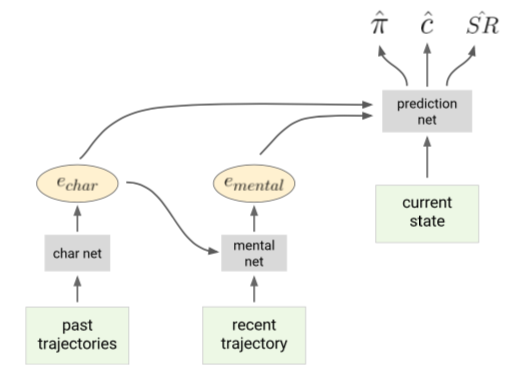
\includegraphics[width=\linewidth, height=\textheight, keepaspectratio]{figs/model}
\label{fig:model}
\caption{\textbf{ToMnet architecture.} Description copied from original paper. The character net parses an agent’s past trajectories from a set of POMDPs to form a character
embedding, $e_{\text{char}}$. The mental state net parses the agent’s trajectory on the current episode, to form an embedding of its mental state, $e_{\text{mental}}$. These embeddings are fed into the prediction net, which is then queried with a current state. This outputs predictions about future behaviour, such as next-step action probabilities ($\hat{\pi}$), probabilities of whether certain objects will be consumed ($\hat{c}$), and predicted successor representations.}
\end{figure}

\noindent \textbf{Experiments} \\[0.15cm]
Only the more complex experiments 3 and 4 are discussed below. In those experiments, ToMnet has to model agents of different \textit{species}, corresponding to different kind of partial observability (i.e. different functions $\omega_i(\cdot)$). Moreover, a subgoal is added to the environment. Agents receive maximum reward for reaching the subgoal location first, then consuming the preferred object that differs from agent to agent. The usefulness of subgoals will become clear when presenting experiment 4.\\

In experiment 3, there are three different species of agents. One species of agent ("blind") can only observe its previous action ($a_{t-1}$) and reward ($r_{t-1}$). The second species has partial observability ("sighted"), but is stateless: these agents can observe the gridworld within a $5 \times 5$ window centered at their current location, with the rest of the maze masked out. The agent policies however are purely reactive (no memory). The third species shares the benefits of the other two, being both sighted and stateful. Figure 3 shows the ToMnet's predictions of future state occupancy for the same query, but given different past observations of how the agent behaves. Without being given the species label, the ToMnet is able to infer it and map out where the agent will go. Indeed, it can be seen that blind agents are predicted to continues until they hit a wall, the second specie has no memory thus consumes objects opportunistically, and sighted stateful agents explore the environment and seek the subgoal. This shows that the model is able to develop general models for the three different species.\\

\begin{figure}[!htb]
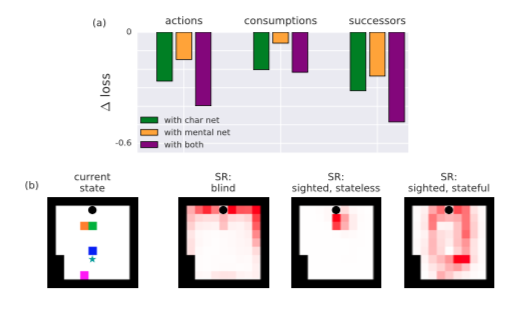
\includegraphics[width=\linewidth, height=\textheight, keepaspectratio]{figs/exp3-1}
\label{fig:exp31}
\caption{\textbf{Using the ToMnet to characterise trained neural-net agents.} Description copied from original paper. \textbf{(a)} Usefulness of ToMnet components for the three behavioural prediction targets, compared with a simple ToMnet with no character nor mental net. Longer bars are better; including both character and mental nets is best. \textbf{(b)} A ToMnet’s prediction of agents’ future state occupancy given a query POMDP state at time $t = 0$ (left). Star denotes the subgoal. The maps on the right are produced after observing behaviour on $N_{\text{past}} = 5$ past POMDPs from a sampled agent of each subspecies (always preferring the pink object). The ToMnet does not know a priori which subspecies each agent belongs to, but infers it from past behaviour.}
\end{figure}

The objective of experiment 4 was to simulate the Sally-Anne test in the gridworld and investigate if ToMnet is able to predict actions of agents possibly holding false beliefs, which is an indicator of a Theory of Mind. The experiment was designed as follows: an agent would see its preferred blue object in one location, but would have to move away in order to reach the subgoal first. During this time, the preferred object is potentially moved by a swap event, which the agent may see if the distance to the subgoal was not greater than its window size. Crucially, ToMnet was able to observe the entire environment and thus aware of swaps when the agent where not. As a result, ToMnet predicted that when the world changes far away from an agent, that agent will continue with a policy that is based on false beliefs. The authors claim that this result validates the fact that ToMnet learns a general Theory of Mind that incorporates an implicit understanding that agents act based on their own persistent representation of the world, even if they are mistaken. \\

\begin{figure}[!htb]
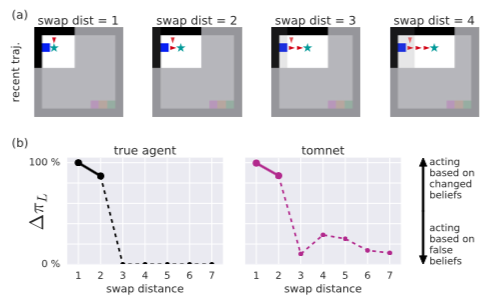
\includegraphics[width=\linewidth, height=\textheight, keepaspectratio]{figs/exp4-2}
\label{fig:exp42}
\caption{\textbf{Sally-Anne test.} Description copied from original paper. \textbf{(a)} We force agents to initially move along a hand-constructed trajectory. Agents have $5 \times 5$ observability and prefer the blue square object, but must seek the subgoal (star) first. When an agent reaches the subgoal, a swap event may or may not occur. If there is no swap, the optimal action is to go left. By extending the length of the path, the swap event will no longer be visible to the agent. (b) Left: effect of a swap event on the agents’ true policies, measured as the relative reduction in their probability of moving back towards the original location where they saw the blue object ($\Delta\pi_L = (\pi(a_L|\text{no swap}) - \pi(a_L|\text{swap}))/\pi(a_L|\text{no swap}) \times 100\%$). If the agent can see that the object has moved from this location (swap dist $\leq$ 2), it will not return left. If it cannot see this location, its policy will not change. Right: ToMnet’s prediction.}
\end{figure}

\section{Discussion}

\noindent In my opinion, one of the main contributions of the authors is that simply by formalizing the problem in the right way, Artificial Theory of Mind can arise. Another strength of this work is the proposed neural network architecture. Using meta-learning introduces some prior about the observed agents which is biologically plausible. Indeed, our brain is often compared to a Bayesian machine by neuroscientist, where the prior is formed from evolution \cite{bayesian-brain}. The advantage of an implicit method such as meta-learning in contrast to more direct ToM Bayesian approaches \cite{dragan, nature} is tmuch lower computational cost.\\

\indent The claim made by the authors that ToMnet succeeded the Sally-Anne test seem to be somewhat exaggerated. Let us do a little bit of self-reflection to explain this. Our thought process when solving the SAT can be split up in three points:
\begin{enumerate}[label=(\arabic*)]
\item Identifying the context, task and actions (Sally puts the ball in the white box \& Anne moves the ball to the other box)
\item Detecting and interpreting gaze cues (Sally does not see Anne moving the ball)
\item Reasoning and drawing conclusions from (1) and (2)
\end{enumerate}
Does ToMnet learn those three skills? It seems to be the case for the first skill. It was in shown in Experiment 3 that ToMnet is able to understand the task and goals of the other agents. On the other hand, we can argue that the second and third skill are more hardcoded than learned in ToMnet. Both the character and mental net have convolution and LSTM layers. It is thus fearly simple for the character net to learn to distinguish the different field of views and for the mental net to determine how far the agent was from the swapped goal. Those two informations are by construction carried to the prediction net. All the prediction net has to do is learn a simple logic verification (field of view $<$ swap distance) to predict a false belief. Eventough, the result of ToMnet are interesting, it is doubtfull that it will generalize that well on a set of tasks with a broader domain.\\

\indent Another shortfall is the SAT itself to test real-life ToM capabilities. A weakness of the Sally-Anne experiment is its passiveness: the observer has no influence on the observed agents. In real-world situations ToM inference is guided by our goals. Risko et al. \cite{risko} show that active observers discover new clues that are not significant in the passive mode. An example of a better experimental ToM setup is found in the work investigated by A. Dragan and her team \footnote{Youtube: An Optimization-Centric Theory of Mind for Human-Robot Interaction}. Her research problem can be described as follows: A person and a drone move together in a small room. The person needs to move from point A to B and the drone from C to D. The segments AB and CD intersect each other. How can the drone make use of observations of the person's behaviour to anticipate its actions? And thus planning a safer navigation. Their model was even more entwined to its context than ToMnet, however the active experimental setup is more challenging and shares more overlap with human-like ToM situations. \\

\indent As mentioned several times, Machine ToM will likely become a core component to construct agents needing to safely interact in multi-agent environments. Another strong advantage of ToMnet referred in \cite{Tomnet}, is to see it as a new tool for interpretability in machine learning. Current techniques in deep learning focus on feature understanding. Whereas, ToMnet can be used to understand other intelligent agents on a more high-level view. In addition, a fascinating scientific application that can be imagined is Artificial ToM agents simulating the evolution of the human's mind. A simulation from past to present could help us better understand why we are like we are. On the other hand, simulating the future societal evolutions is also interesting yet more speculative. To conclude, with all great technological progress comes an other side to the coin. Technological manipulation - think social media posts and the U.S. presidential campaign of 2016 - could be worsened if A.I. is capable of detecting and acting on false beliefs.



% ==============================================================================

\bibliographystyle{unsrt}
\bibliography{bibliography.bib}

\end{document}